\documentclass[notes]{beamer}

\usepackage{default}
\usepackage{pgfpages}

\usetheme{Szeged}
\usecolortheme{dolphin}

\title{Extensions on Contract Net Protocol for AGVs}
\subtitle{Multi-Agent Systems}

\author{\textbf{Jens Claes} \and Victor Le Pochat}
\date{June 6, 2016}

\setbeamertemplate{note page}{\pagecolor{yellow!15}\insertnote}
\setbeameroption{hide notes} % Only slides
\newcommand{\seperation}{\vspace{0.5cm}\hrule\vspace{0.5cm}}
%\setbeameroption{show notes on second screen=right} % Both

\graphicspath{ {../verslag/images/} }

\begin{document}
	\frame{\titlepage}

	\section{Introduction}
	
	\begin{frame}{Objectives \& Hypotheses}
		\begin{itemize}
		\item CNET vs CNCP vs DynCNET
		\item Hypotheses:
			\begin{itemize}
			\item Compare
				\begin{itemize}
				\item Profit
				\item Delivery time
				\item \# clients undelivered
				\item Message count
				\end{itemize}
			\item Influence on profit
				\begin{itemize}
				\item \# drones
				\item \# warehouses
				\item \# clients
				\end{itemize}
			\end{itemize}
		\end{itemize}
	\end{frame}
	\note{Hypotheses zelf gewoon zeggen}
		
	\section{Design}
	\begin{frame}{Setting}
		\begin{itemize}
		\item Package delivery company
		\item Drones (UAV)
		\item Battery-constrained
		\item Crashes (Poisson-distributed)
		\item Warehouses
		\item 2 types clients
		\item Fines
		\end{itemize}
	\end{frame}
	
%	\begin{frame}{MAS design}
%		\begin{itemize}
%			\item Clients have an order
%			\item Drone takes up order
%			\item Drone collects package at warehouse
%			\item Drone flies to client and delivers package
%		\end{itemize}
%	\end{frame}
	
	\begin{frame}{MAS design}
		\begin{itemize}
			\item Maximize profit company
			\item Allocate task to most suitable drone
			\item Find cheapest warehouse
			\item Minimize crashes
			\note{Minimize crashes by recharging in warehouse mid delivery}
			\item Deliver on time
			\item Cost estimation
				\begin{itemize}
				\item Price package
				\item Price battery charge
				\item Price failed drone
				\item Price client
				\end{itemize}
		\end{itemize}
	\end{frame}

	\section{Protocols}
	\begin{frame}{Contract Net Protocol (CNET)}
		\begin{itemize}
			\item Contract negotiation
			\linebreak
			\begin{tabular}{cl}
				M & Task announcement \\
				C & Bid (on best) \\
				M & Awarding \\
				C & Execution \\
			\end{tabular}
			\seperation
			\item Only announce order\note{Not bid deadline etc}
			\item Only 1 outstanding bid
			\item Implemented RefusalReason (+ nextAvailableTime)
		\end{itemize}
	\end{frame}

	\begin{frame}{Contract Net with Confirmation (CNCP)}
		\begin{itemize}
			\item Delayed commitment
			\item Bid on all
			\item Accept/Decline when awarded
			\seperation
			\item 1 message
			\item Reannounce task
		\end{itemize}
	\end{frame}

	\begin{frame}{Dynamic Contract Net (DynCNET)}
		\begin{itemize}
			\item Allow contract switching
				\begin{itemize}
				\item Manager
				\item Contractor
				\end{itemize}
			\item Preparation vs execution
			\seperation
			\item No oscillation prevention
		\end{itemize}
	\end{frame}
	
	\begin{frame}{Other extensions}
		\begin{itemize}
			\item Prebidding vs Definitive bidding (Aknine et al.)
			\item Iterated Contract Net
			\item Leveled commitment
		\end{itemize}
	\end{frame}
	
	\section{Experiments}
	\begin{frame}{Experiment Setup}
		\begin{itemize}
			\item 2 experiments
				\begin{enumerate}
				\item Vary \# drones/warehouses/clients
				\item 10 drones, warehouses; vary \# clients
				\end{enumerate}
			\item 150 repetitions
			\item ANOVA
			\item Games-Howell vs TukeyHSD
		\end{itemize}
	\end{frame}
	\begin{frame}{Experiment Results (Profit)}
		\begin{columns}[c]
			\column{.6\textwidth}
			\begin{itemize}
				\item All profitable
				\item CNCP
					\begin{itemize}
					\item Few drones: Similar CNET, slightly better
					\item Many drones: A lot better than CNET
					\end{itemize}
				\item DynCNET
				\begin{itemize}
					\item Few drones: breaks down
					\item Many drones: Most profitable of all
				\end{itemize}
			\end{itemize}
			
			\column{.4\textwidth}
			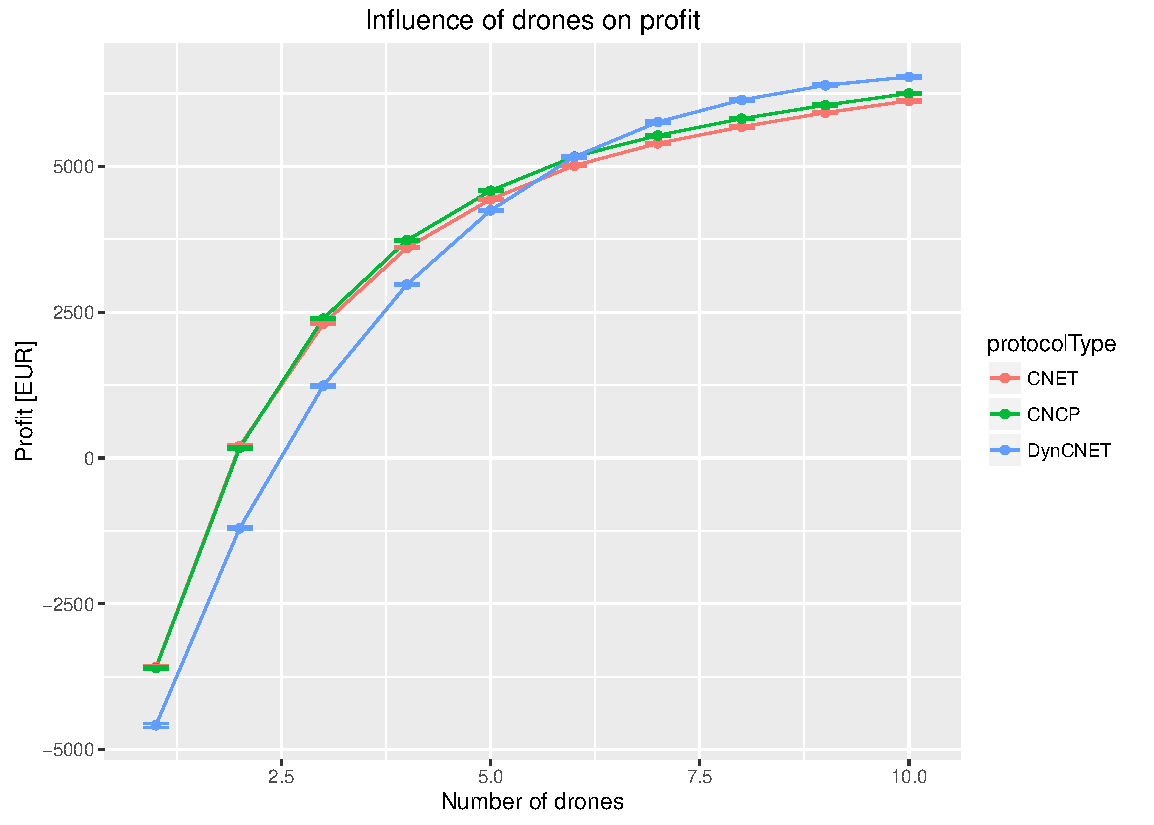
\includegraphics[width=\columnwidth]{drones-profit}
		\end{columns}
	\end{frame}
	\begin{frame}{Experiment Results (Rest)}
		\begin{columns}[c]
			\column{.6\textwidth}
			\begin{itemize}
				\item Delivery time: $CNCP < CNET < DynCNET$
				\item \# clients not delivered: $CNCP < CNET$, complex
				\item \# messages: $CNET < CNCP << DynCNET$
			\end{itemize}
			
			\column{.4\textwidth}
			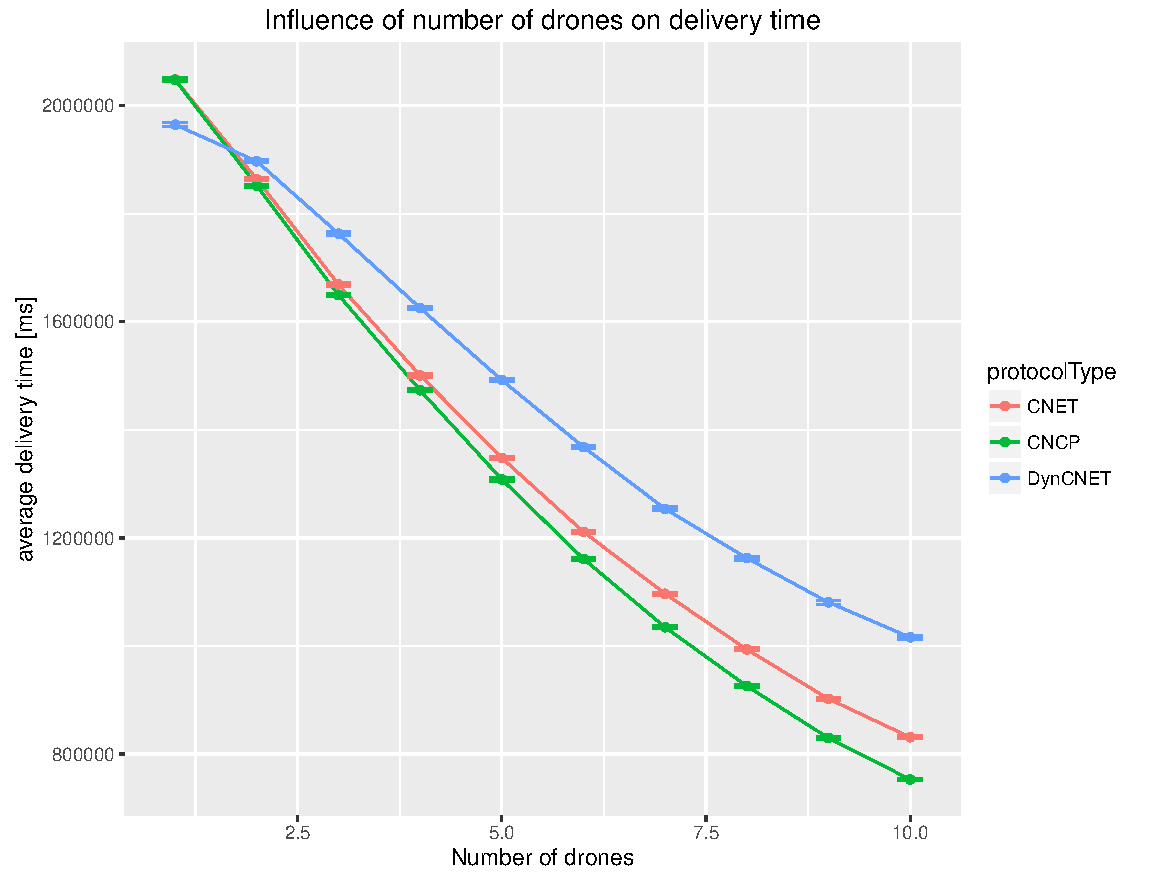
\includegraphics[width=\columnwidth]{drones-deliverytime}
		\end{columns}
	\end{frame}
	
	\section{Conclusion}
	\begin{frame}{Conclusion}
		\begin{itemize}
			\item Both improve upon CNET
			\item CNCP
				\begin{itemize}
				\item Few drones: best
				\item Few drawbacks
				\end{itemize}
			\item DynCNET
				\begin{itemize}
				\item Many drones: best
				\item A lot more messages
				\item Oscillation prevention necessary
				\end{itemize}
		\end{itemize}
	\end{frame}
	
\end{document}
